\section{Auswertung}
\label{sec:Auswertung}
Für die Untersuchung der verschiedenen aufgenommenen $\gamma$-Spektren werden die Kanäle des ``ADC'' auf die entsprechenden Energien kalibriert. Desweiteren wird die Effizienz des Detektors exemplarisch an dem Eu-Spektrum berechnet und anschließend die Messwerte zur Bestimmung der Aktivität der verwendeten Bariumquelle mit ihr bereinigt. Desweiteren wird das Compton-Kontinum sowie der Photopeak einer Cs-Quelle untersucht, sowie geprüft ob der Photopeak Gaußverteilt ist. Zuletzt wird anhand des Spektrums versucht auf die Zerfallsprodukte eines Minerals zu schließen und somit deren Zerfallskette zu bestimmen.


\subsection{Kalibrieren des Detektors anhand $^{152}$EU Spektrums}
Zum Kalibrieren des Detektors wird im folgenden die Kanalnummer entsprechenden Energien zugewiesen, sowie die Effizenz des Detektors bestimmt.


\subsubsection{Energiekalibrierung}
Zunächst wird die Kanalnummer auf die Energie anhand des Spektrums des EU$^{152}$ Strahlers kalibriert. Die Energie mit den entsprechenden Kanalnummern sind in Tabelle \ref{tab:CsSpekt} aufgeführt.

\begin{table}
  \centering
  \caption{Kenngrößen eines $^{152}$Eu-Strahlers, sowie des Detektors}
  \begin{tabular}{c | c c c c}
    \toprule
    Energie $E_{\gamma}$ / keV& Kanal & Emissionwahrscheinlichkeit / \% & Counts & Effizienz / \% \\
    \hline
    121.78	& 403	& 28.6	& 3078 	& ---	\\
    244.70	& 803	& 7.6	& 485 	& \num{10.40 +- 0.1}	\\
    344.30	& 1128	& 26.5	& 1048	& \num{6.40 +- 0.1}	\\
    411.12	& 1345	& 2.2	& 79	& \num{5.80 +- 0.1}	\\
    443.96	& 1452	& 3.1	& 112 	& \num{5.90 +- 0.1}	\\
    778.90	& 2544	& 12.9	& 193	& \num{2.44 +- 0.04}	\\
    867.37	& 2832	& 4.2	& 61	& \num{2.36 +- 0.03}	\\
    964.08	& 3147	& 14.6	& 132	& \num{1.47 +- 0.02}	\\
    1085.90	& 3543	& 10.2	& 88	& \num{1.40 +- 0.02}	\\
    1112.10	& 3629	& 13.6	& 108	& \num{1.29 +- 0.02}	\\
    1408.00	& 4593	& 21.0 	& 134	& \num{1.04 +- 0.02}	\\
    \bottomrule
  \end{tabular}
  \label{tab:CsSpekt}
\end{table}

Um die Korrelation zwischen der Energie und der Kanalnummer zu bestimmen wird eine lineare Regression durch die Tupel aus Energie und Kanalnummer gelegt. Das Ergebniss ist in Abbildung \ref{fig:RegCs} zu sehen.

\begin{figure}[htpb]
  \centering
  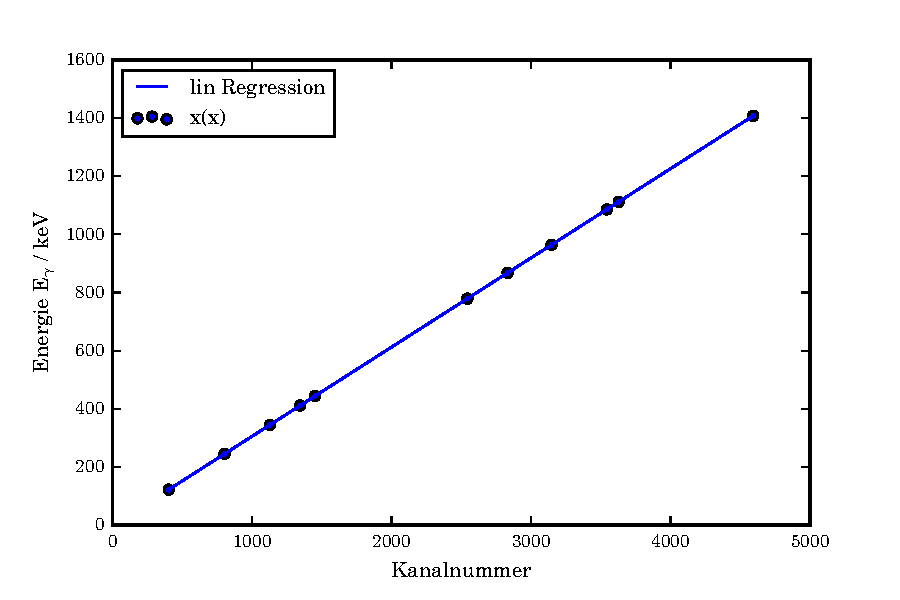
\includegraphics[width=\textwidth]{./build/CsReg.pdf}
  \caption{Lineare Regression zur Bestimmung der Korrelation zwischen Kanalnummer und $\gamma$-Quantenenergie}
  \label{fig:RegCs}
\end{figure}

Aus der Regression ergibt sich eine Energiedifferenz zweier benachbarter Kanäle beträgt von
\begin{equation}
  \Delta E = (\num{306.97 +- 0.03}) \, \text{keV}
  \label{eqn:Reg}
\end{equation}
Anhand der Energieskala werden die gemessenen Counts im weiteren in Abhängikeit der $\gamma$-Quanten Energie $E_{\gamma}$ dargestellt.


\subsubsection{Effizienzbestimmung}
\label{sec:Q}
Das für den Eu-Strahler aufgenommene Spektrum ist in Abbildung \ref{fig:SpekCs} zu sehen.

\begin{figure}[htpb]
  \centering
  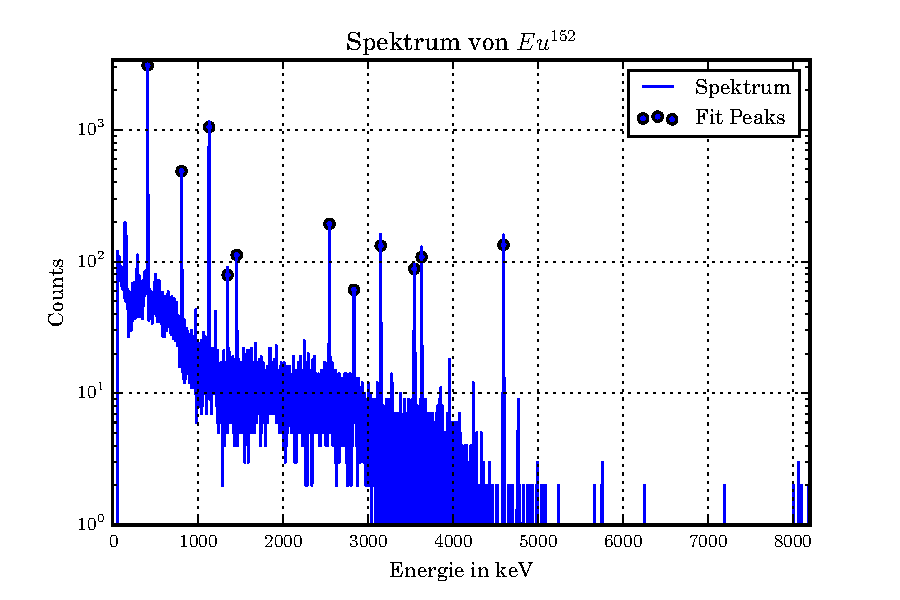
\includegraphics[width=\textwidth]{./build/SpektEu.pdf}
  \caption{<+caption text+>}
  \label{fig:SpekCs}
\end{figure}

Die Aktivität $A_\text{Eich}$ der verwendeten Europium Isotop betrug am 01.10.2000
\begin{equation}
  A_\text{Eich} = (\num{4130 +- 60}) \, \text{Bq}
  \label{eqn:AktEu}
\end{equation}
und die Halbwertszeit
\begin{equation}
  \tau_{1/2} = (\num{4943 +- 5}) \, \text{Tage} \ .
  \label{eqn:halb}
\end{equation}
Anhand Formel \ref{eqn:??} lässt sich mittels der Zeitdifferenz zwischen der geeichten Aktivität und dem am Tag der Durchführung der Messung (09.01.2017) eine Aktivität von
\begin{equation}
  A_\text{Durch} = (\num{1242 +- 35}) \, \text{Bq}
  \label{eqn:AktEEu}
\end{equation}
berechnen. Dem Versuchsaufbau wird ein Abstand $a$ zwischen Quelle und Detektor von
\begin{equation}
  a = 8.8 \, \text{cm}
  \label{<++>}
\end{equation}
und ein Radius $r$ des Detektors von
\begin{equation}
  r = 2.25 \, \text{cm}
  \label{<++>}
\end{equation}
gemessen. Aus diesen lässt sich durch einsetzen in Formel \ref{eqn:??} ein Raumwinkel $\Omega$ von
\begin{equation}
  \Omega = 0.196
  \label{eqn:Raum}
\end{equation}
berechnen. Der Raumwinkel $\Omega$ ist jedoch nur unter vorbehalt zu verwenden, da der Abstand zwischen Quelle und Detektor kleiner als 10 cm ist und dies nicht mehr im gültigkeitsbereich der Formel \ref{eqn:??} liegt. Aus dem Raumwinkel $\Omega$, der Wechselwirkungswahrscheinlickeit $W$, der Aktivität $A_\text{Durch}$ sowie die effektive Messzeit lässt sich nach Formel \ref{eqn:??} die Effizienz $Q$ berechnen. Die Ergebnisse in Abhängikeit der Energie sind in Tabelle \ref{tab:CsSpekt} aufgeführt. Um die Effizienz in den folgenden Auswertungsteil \ref{sec:??} zur berücksichtigen, wird die Effizenz in erster Näherung durch ein Potenzfunktion dargestellt.

\begin{figure}[H]
  \centering
  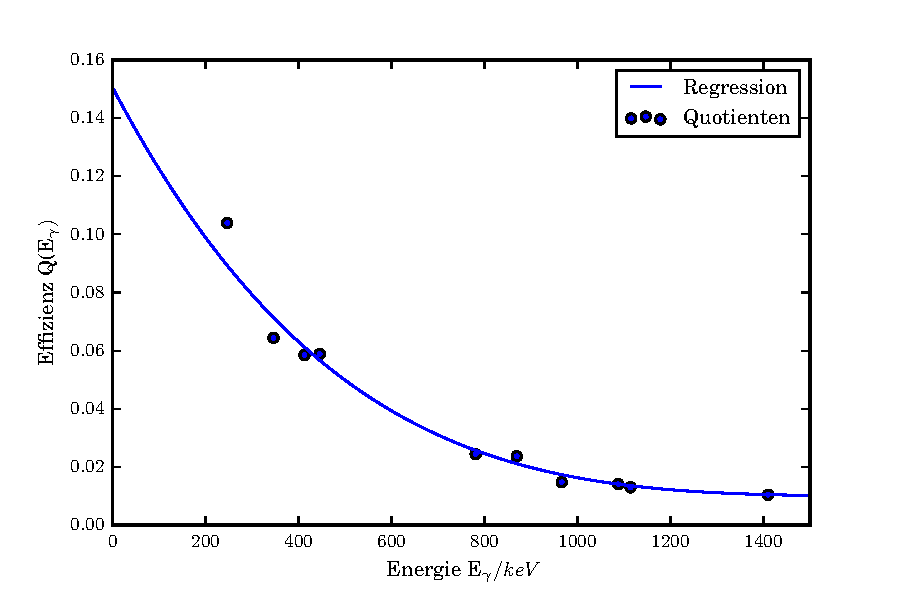
\includegraphics[width=\textwidth]{./build/Effizienz.pdf}
  \caption{Effizienz des verwendeten Germaniumdetektors}
  \label{fig:Efi}
\end{figure}

Die ermittelte Potenzfunktion zur berechnung der Effizienz in Abhängigkeit der Energie, hat die Form
\begin{equation}
  Q(E_\gamma)= 1.2 \cdot 10^{-14} \left( x - 1850 \right)^4 + 0.01 \ .
  \label{eqn:QCs}
\end{equation}


\subsection{$^{137}$Cs-Strahler}
Zunächst wird die Laage des Photopeaks bestimmt und das Compton-Kontinum genauer untersucht . Anschließend wird geprüft ob der Photopeak einer Gaußverteilung entspricht. Zuletzt wird die Absorptionswahrscheinlichkeit des Detektors berechnet und erklärungen für die Gestalt des Compton-Kontinums, sowie des Photopeaks gesucht.


\subsubsection{Photopeak}
In dem Aufgenommenen Spektrum wird mittels der Funktion find\_peaks\_cwt aus der numpy Biblothek die Laage des Photopeaks bestimmt. Das Ergebniss ist in Abbildung \ref{fig:SpekCs} zu sehen.

\begin{figure}
  \centering
  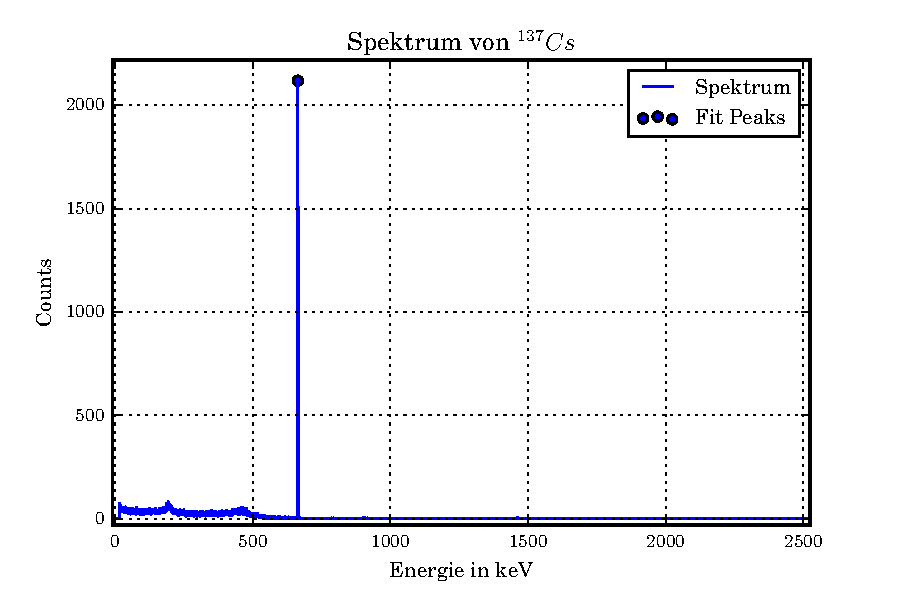
\includegraphics[width=\textwidth]{./build/SpektCS.pdf}
  \caption{Spektrum des Cs-Strahlers}
  \label{fig:SpekCS}
\end{figure}

Dabei wurde die X-Achse schon mittels der in Auswertungsteil \ref{sec:} Energie skaliert. Der Photopeak wird bei Energie von
\begin{equation}
  E_\gamma = 663 \, \text{keV}
  \label{eqn:CsPhoto}
\end{equation}
detektiert. Im späteren Teil der Auswertung wird geprüft ob der Photopeak einer gaußförmigen Verteilung zu Grunde liegt.


\subsubsection{Compton-Kontinum}
Für die weiteren Rechnungen wird zunächst die natürliche Energie $\varepsilon$ nach Formel \ref{eqn:??} eingeführt, welche
\begin{equation}
  \varepsilon = 1.292
  \label{eqn:nE}
\end{equation}
beträgt. Aus der natürlichen Energie $\varepsilon$ des Strahlers kann die theoretische Laage der Comptonkante $E_\text{ComKan, theo}$ nach Formel \ref{eqn:??} berechnet werden. Sie beträgt
\begin{equation}
  E_\text{ComKan, theo} = 478 \, \text{keV}
  \label{eqn:KanTheo}
\end{equation}
Das Spektrum im bereich des Compton-Kontinums ist in Abbildung \ref{fig:Compt} zu sehen.

\begin{figure}[htpb]
  \centering
  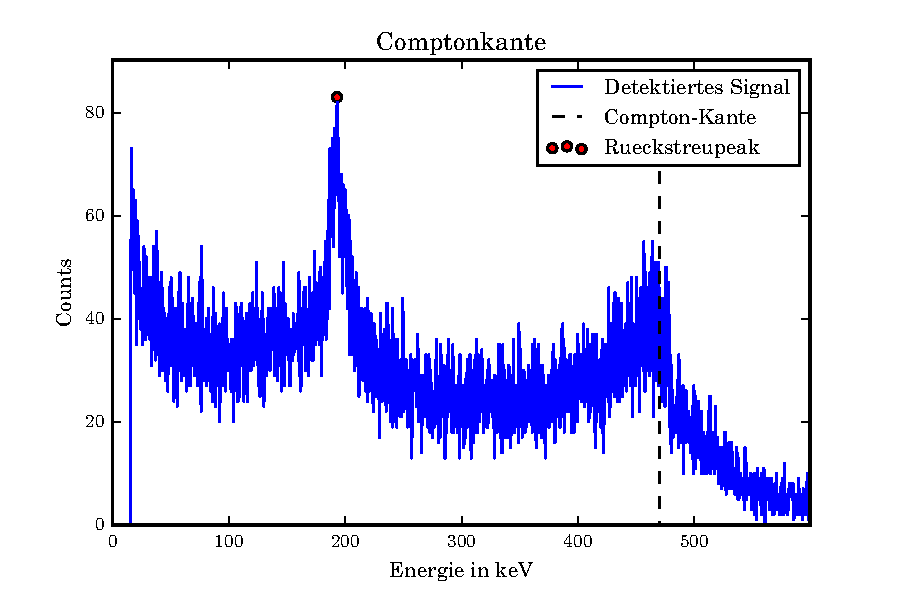
\includegraphics[width=\textwidth]{./build/Compton.pdf}
  \caption{Compton-Kontinum mit Rückstreupeak und maximalen Energieübertrag}
  \label{fig:Compt}
\end{figure}

Aus ihm wird ein Rückstreupeak von
\begin{equation}
  E_\text{rück} = 193 \, \text{keV}
  \label{eqn:KanExp}
\end{equation}
und die Energie der maximalen Energieübertragung von
\begin{equation}
  E_\text{l,max} = 470 \, \text{keV}
  \label{eqn:RückExp}
\end{equation}
abgelesen.


\subsubsection{Verteilung des Photopeaks}
Um zu überprüfen ob der Photopeak gaußverteilt ist wird der Zusammenhang zwischen der Zehntelwertsbreite und der Halbwertsbreite überprüft. Dazu wird zunächst das Maximum $M$ bestimmt. Anschließend wird eine Linie in die Messwerte gelegt die dem $M/n$ fachen entspricht. Zwischen den jeweiligen Werten die am nächsten an der Linien des $M/n$ fachen liegt wird eine lineare Regression durchgeführt und der Punkt bestimmt bei dem die Regression den Wert $M/n$ angenommen hatt. Die Punkte werden jeweils für die Seite links und rechts vom Maximum bestimmt und der Abstand dortzwischen ermittelt. Der Abstand wird als $1/n$-Wertsbreite bezeichnet.
Die Halbwertsbreite sowie die Zehntelwertsbreite sind in Abbildung \ref{fig:Halb} zu sehen.

\begin{figure*}[htpb]
	\centering
	\begin{subfigure}[t]{0.5\textwidth}
		\centering
		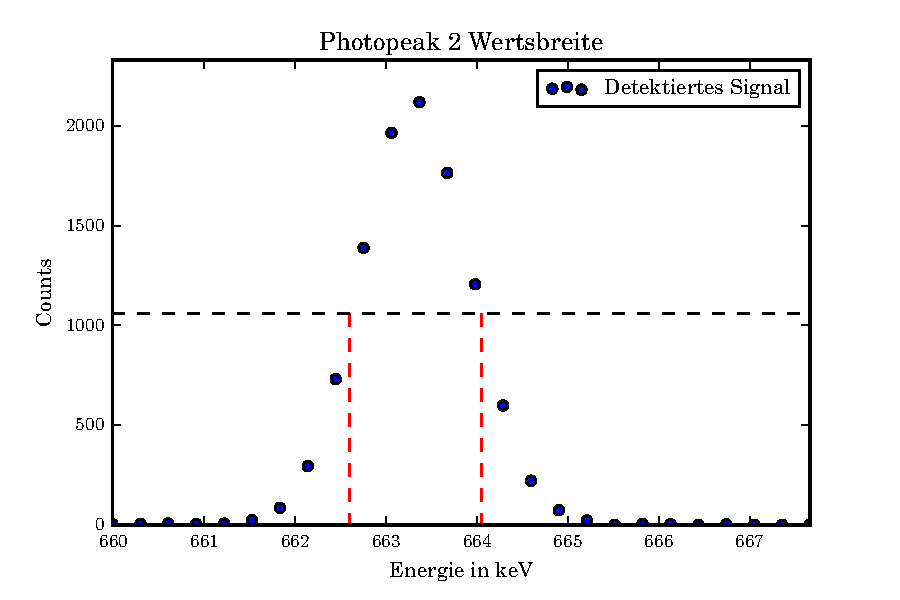
\includegraphics[width=\textwidth]{./build/2Wertsbreite.pdf}
		\caption{Halbwertsbreite}
	\end{subfigure}%
	\begin{subfigure}[t]{0.5\textwidth}
		\centering
		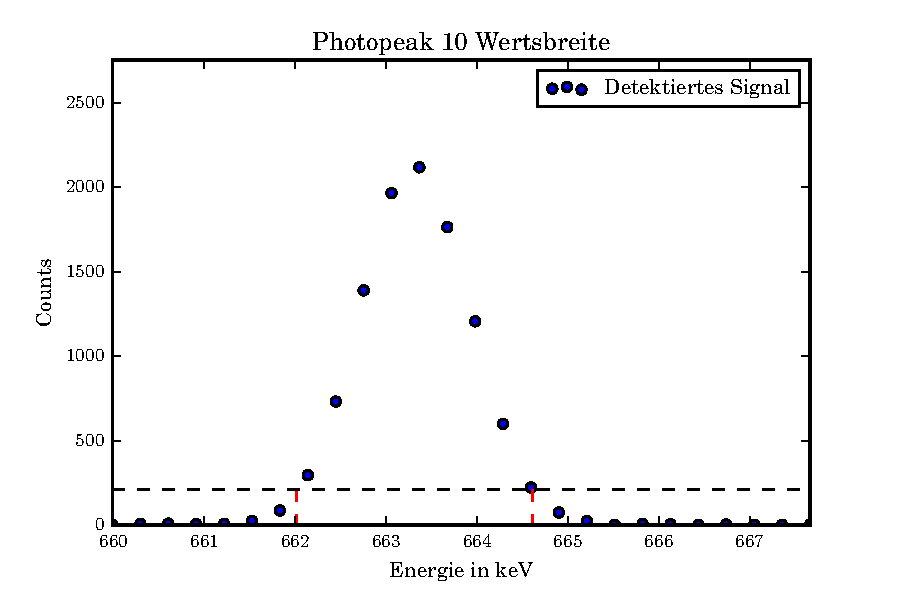
\includegraphics[width=\textwidth]{./build/10Wertsbreite.pdf}
		\caption{Zehntelwertsbreite}
	\end{subfigure}
	\caption{Caption place holder}
	\label{fig:Halb}
\end{figure*}

Die ermittelte Halbwertsbreite $E_{1/2}$ beträgt
\begin{equation}
  E_{1/2} = 1.46 \, \text{keV}
\end{equation}
und die Zehntelwertsbreite $E_{1/10}$ beträgt
\begin{equation}
  E_{1/10} = 2.60 \, \text{keV}
\end{equation}
Im Falle einer Gaußverteilung müsste das Verhältniss zwischen Halb- und Zehntelwertsbreite
\begin{equation}
  E_{1/10} = 1.823 E_{1/2}
\end{equation}
seien. Das Verhältniss zwischen den experimentell Bestimmten breiten ist
\begin{equation}
  E_{1/10} = 1.78 E_{1/2}
  \label{eqn:Ver}
\end{equation}
Daraus wird geschlossen das hinreichend viele Werte genommen worden sind, sodass die Poissonverteilung in die Gaußverteilung übergeht.

\subsubsection{Absorptionswahrscheinlichkeit im Detektor}
Aus Abbildung \ref{fig:??} kann der Extinktionskoeffizient $\mu$ in abhängigkeit von Germanium entsprechend der auftretenden Effekte abgelesen werden . Der Extinktionskoeffizient beim Photoeffekt bei einer Energie von ~650 keV ist in etwa
\begin{equation}
  \mu_\text{Photo} = 0.002 \, \text{cm} ^{-1} \ .
  \label{eqn:muPhoto}
\end{equation}
Unter Verwendung von Formel \ref{eqn:??} lässt sich die Absorptionswahrscheinlichkeit durch den Photoeffekt auf
\begin{equation}
  W_\text{Absorp, Photo} = 0.5 \, \%
  \label{eqn:AbsorpPhoto}
\end{equation}
berechnen. Der Extinktionskoeffizient beim Comptoneffekt bei ~650 keV beträgt
\begin{equation}
  \mu_\text{Compt} = 0.4 \, \text{cm} ^{-1} \ .
  \label{eqn:muCompt}
\end{equation}
Daraus errrechnet sich eine Absorptionswahrscheinlichkeit von
\begin{equation}
  W_\text{Absorp, Compton} = 70 \, \% \ .
  \label{eqn:AbsorpComp}
\end{equation}
Eine mögliche Erklärung dafür, dass der Photopeak dennoch im Spektrum so hoch ausfällt könnte seien, dass der Extinktionskoeffizient in dem Abschirmmaterial deutlich größer ist. Die Elektronen könnten möglicherweise mit aufgrund ihrer kinetischen Energie zwar aus dem Aluminium herausgelöst werden, aber erst in der Sperrschicht detektiert.
\subsection{Aktivitätsbestimmung der verwendeten $^{133}$Ba-Quelle}
Die Intensitäten der Spektrallinien $Z$ und die Wechselwirkungswahrscheinlickeit $W$ sind in Tabelle \ref{tab:Ba} zusammen mit den kalibrierten Energien aufgetragen. Der Raumwinkel wurde bereits in Kapitel \ref{sec:Q} bestimmt und beträgt $\Omega$ = 0.19.
\begin{table}
  \centering
  \caption{Aktivität in Abhängigkeit der Energie sowie der Effizienz und der Wechselwirkungswahrscheinlichkeit}
  \begin{tabular}{c c c c}
    \toprule
	Energie $E_\gamma$ \ keV & Intensität $Z$ & Wechselwirkungsw. / \% $W$ & Aktivität $A$ \\
    \hline
	82	& 3177	& 34.1	& 1307	\\
	162	& 144	& 0.6	& 3994	\\
	304	& 918	& 18.3	& 1142	\\
	357	& 2509	& 62.1	& 1038	\\
	389	& 320	& 8.9	& 995	\\
    \bottomrule
  \end{tabular}
  \label{tab:Ba}
\end{table}
Durch umstellen der Gleichung \ref{eqn:??} nach A lässt sich die Aktivität der Probe ermitteln wobei die Zählergebnisse noch einmal durch die Messdauer geteilt werden müssen. Die Lifetime des Detektors beträgt 3595 s. Die Aktivitäten der einzelnen Energien sind in Tabelle \ref{tab:Ba} aufgetragen. Das gemittelte Ergebniss beträgt
\begin{equation}
  (\num{1120 +- 30}) \, \text{Bq}
  \label{eqn:aktBq}
\end{equation}
wobei die Aktivität der Messunf mit der Energie von 162 keV vernachlässigt wurde, da der Messfehler bei der geringen Aktivität, verhältnissmäßig groß in anbetracht der anderen Aktivitäten scheint.
\subsection{Zerfallsreihe des unbekannten Minerals}
Es wird versucht aus dem Linienspektrum des verwendeten Minerals auf die Zerfallsreihe der Probe zu schließen. Das Linienspektrum des Minerals ist in Abbildung \ref{fig:Stone} zu sehen.
\begin{figure}[htpb]
  \centering
  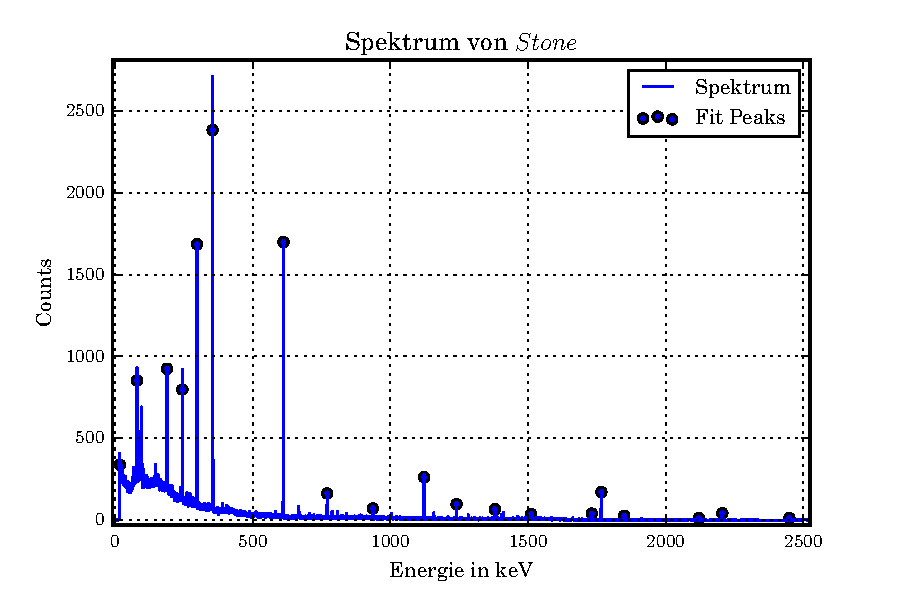
\includegraphics[width=\textwidth]{./build/SpektSt.pdf}
  \caption{Spektrum von verwendeten Mineral}
  \label{fig:Stone}
\end{figure}
Bei dem Vergleich mit der $^{238}$Uran-Zerfallsreine fällt auf das das die Isotope von $^{236}$Ra bis $^{210}$Bi$^\text{m}$ alle auftreten. Dabei wird der Zerfall von $^{210}$Pb jedoch aufgrund der langen Halbwertszeit im vergleich zur Versuchdauer nicht detektiert.
